%\newpage
\section{Architettura}
\subsection{Descrizione generale}
Per la realizzazione del componente si è deciso di utilizzare un approccio comportamentale(behavioral).
L'architettura realizzata consiste in un unico modulo che realizza la macchina a stati finiti, escludendo il modulo della RAM che viene fornito dal TestBench.\\
Il modulo utilizza al suo interno due processi sincronizzati:"stato" e "combin".
Il processo "stato" è sincronizzato sul fronte di salita del clock e si occupa di aggiornare lo stato corrente della macchina.Si è scelto di aggiornare lo stato sul fronte di salita in quanto anche la RAM aggiorna i propri segnali alla salita del clock, dunque si mantiene una coerenza in fase di aggiornamento. \\
Il processo "combin", sincronizzato sul fronte di discesa del clock, implementa la macchina a stati vera e propria, ovvero quello che la macchina deve fare in base al suo stato corrente.

\subsubsection{Ipotesi}
Essendo il periodo di clock pari a 100 ns si è ipotizzato che il tempo di transazione del valore dei segnali sia minore di metà periodo di clock. In questo modo il processo "combin" può leggere i valori corretti dei segnali e decidere il prossimo stato.\\
In fase di sperimentazione questa ipotesi è stata verificata come corretta.

\subsection{Macchina a stati}
In figura \ref{fig:macchina_stati} viene riportato il diagramma della macchina a stati.\\

%c'è da cambiare start_attendi in start_wait
\begin{figure}
    %\centering
    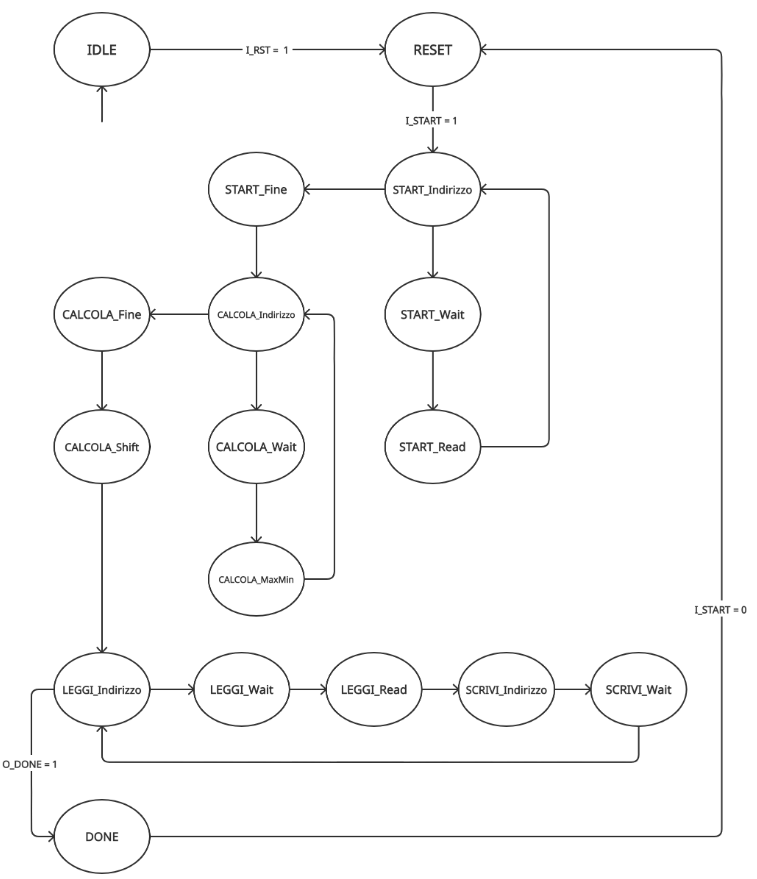
\includegraphics[width = 15 cm]{Immagini/Diagramma degli stati.png}
    \caption{Diagramma degli stati del componente}
    \label{fig:macchina_stati}
\end{figure}

\subsubsection{Descrizione macchina}
La macchina è composta dai seguenti stati:\\

\begin{itemize}
    \item IDLE : stato iniziale della macchina nel quale vengono inizializzati tutti i segnali e le variabili utilizzate.La macchina rimane in questo stato fino a quando non riceve il primo segnale di reset(i\_rst = 1), il quale fa passare la macchina nello stato di RESET.
    
    \item RESET : in questo stato la macchina aspetta il segnale di inizio codifica, ovvero aspetta che il segnale i\_start venga messo uguale a 1. Questo vuol dire che l'immagine in memoria è pronta ad essere codificata e la macchina inizia l'elaborazione passando allo stato successivo.
    
    \item START\_Indirizzo : la macchina si prepara a leggere dalla memoria il numero di colonne(byte 0) e il numero di righe(byte 1) settando o\_en = 1, o\_we = 0 e o\_address pari all'indirizzo 0 nel caso di prima iterazione o pari all'indirizzo 1 nel caso di seconda interazione. Se la macchina non ha ancora letto entrambe le dimensioni allora lo stato successivo sarà START\_Wait, altrimenti si prosegue con START\_Fine.
    
    \item START\_Wait : questo stato serve alla macchina per aspettare un ciclo di clock necessario alla memoria RAM per settare correttamente il segnale i\_data con l'informazione presente al byte richiesto dal componente.
    
    \item START\_Read : in questo stato viene effettivamente letta la risposta della RAM alla richiesta e viene memorizzata come numero colonne o numero di righe a seconda dell'indirizzo richiesto.Da questo stato si torna poi a START\_Indirizzo.
    
    \item START\_Fine : qui la macchina salva il numero totale di bit come prodotto dei dati precedentemente letti e si prepara per leggere tutti i pixel dell'immagine per trovare il massimo e minimo valore presente.
    
    \item CALCOLA\_Indirizzo : fino a quando la macchina non ha letto i valori di tutti i pixel setta o\_address con il prossimo indirizzo da leggere e poi passa allo stato CALCOLA\_Wait.Se invece ha già letto tutti i pixel passa a CALCOLA\_Fine.
    
    \item CALCOLA\_Wait : analogo a START\_Wait con la sola differenza nello stato prossimo che sarà CALCOLA\_MaxMin.
    
    \item CALCOLA\_MaxMin : la macchina legge il valore richiesto e lo confronta con il massimo e minimo trovati fino a quel momento,aggiornandoli se necessario.
    
    \item CALCOLA\_Fine : è finita la lettura e valutazione di tutti i pixel e dal prossimo stato inizia l'algoritmo di elaborazione dell'immagine vero e proprio.
    
    \item CALCOLA\_Shift : si calcola il delta e, tramite un semplice controllo a soglia, si determina il valore dello shift, quindi si realizzano le formule \eqref{delta} e \eqref{shift}.
    
    \item LEGGI\_Indirizzo : la macchina deve leggere di nuovo dalla RAM tutti i pixel per convertirli uno ad uno e, fino a quando non li ha elaborati tutti, setta il segnale o\_address all'indirizzo successivo e passa allo stato LEGGI\_Wait.Se invece li ha già convertiti tutti vuol dire che la computazione dell'immagine è terminata, dunque pone ad un valore alto il segnale o\_done e passa allo stato DONE.
    
    \item LEGGI\_Wait : si aspetta il ciclo di clock necessario alla RAM come nei casi precedenti.
    
    \item LEGGI\_Read : si legge il valore effettivo del pixel richiesto e lo si converte applicando l'algoritmo descritto nell'introduzione per il calcolo del nuovo pixel da inserire, in particolare formule \eqref{temp} e \eqref{new}.
    
    \item SCRIVI\_Indirizzo : si prepara la memoria per scrivere, quindi o\_en = 1 e o\_we = 1, inserendo in o\_address l'indirizzo nel quale scrivere il pixel N-esimo, come descritto nella formula \eqref{posizione}.
    
    \item SCRIVI\_Wait : si aspetta un ciclo di clock per attendere che il nuovo valore venga correttamente memorizzato in memoria;dopo questo stato si torna a LEGGI\_Indirizzo.
    
    \item DONE : in questo stato la macchina ha terminato l'elaborazione dell'immagine e aspetta che il segnale i\_start venga abbassato.Quando questo accadrà passa allo stato successivo, ovvero torna allo stato RESET in quanto deve essere pronta per una nuova esecuzione appena il segnale i\_start diventerà di nuovo alto, senza aspettare il RESET.
\end{itemize}

\subsubsection{Note generali sul funzionamento della macchina}
Alcuni dettagli generali:\\
\begin{itemize}
    \item Il segnale di fine computazione o\_done è sempre pari a 0 tranne quando la macchina ha finito l'elaborazione, in particolare viene posto a 1 dallo stato LEGGI\_Indirizzo e poi verrà mantenuto tale dallo stato DONE, per poi essere abbassato nuovamente quando i\_start viene posto a 0, cioè quando torna allo stato RESET.
    
    \item La macchina a stati utilizzata ovviamente non è minima infatti, effettuando delle ottimizzazioni, sarebbe possibile aggregare più stati, per esempio tutti gli stati che terminano con X\_Wait. 
    Essendo il numero di FF e di LUT utilizzato molto minore di quelli disponibili complessivamente ed essendo ampiamente rispettato il vincolo sul tempo di clock di 100 ns, si è deciso di utilizzare la macchina non ottimizzata in favore di una maggior leggibilità del codice e stati più semplici.
    
    \item Il reset è asincrono, ovvero in qualsiasi momento viene posto a 1 il segnale i\_rst il processo "combin" si attiva e pone a 1 il segnale interno resetAttivato, che verrà utilizzato nel processo "stato" al prossimo fronte di salita per un aggiornamento sincrono dello stato. Per semplicità nella figura \ref{fig:macchina_stati} non è stato riportato, ma l'aggiornamento dovuto al reset è indipendente dallo stato corrente della macchina, ovvero in qualunque stato essa sia al fronte di salita successivo lo stato corrente sarà RESET.Inoltre, per come è stata progettata la macchina, se a seguito del reset il segnale i\_start viene lasciato pari ad 1 verrà iniziata una nuova elaborazione della stessa immagine.Se invece c'è la necessità di cambiare i dati in memoria allora occorre porre a 0 i\_start quando il reset viene attivato.

\end{itemize}


























